\chapter{Derivation of Ramsey's Method~\cite{NMR_Notes}}
% \textbf{MUST BE EDITED}
Here is a review of the Ramsey technique for the molecular beam
resonance experiments. In previous studies, the oscillating fields
were extended uniformly throughout the regions in which the energy
levels of the system were investigated.  This was not efficient since
the amplitude and the phase of the oscillating field might change
along the path of the beam. As a different approach, Ramsey suggested
to confine the oscillating fields to small regions; one at the
beginning of the space which the energy levels are being studied and
the other one at the end. In this case, there is no oscillating field
in between.

Consider a system which is subjected to an oscillatory perturbation at
time $t_1$. This induces a transition between the eigenstates p and q:
\begin{equation}
V=
\left(
\begin{array}{cc}
0 & \hbar b e^{i\omega t} \\ 
\hbar b e^{-i \omega t} & 0
\end{array} 
\right)
\end{equation}
An example of such perturbation is a system with a magnetic moment
entering a region with rotating magnetic field with angular velocity
$\omega$. The general wave function for this system is
\begin{equation}
\psi(t)= C_p (t) \psi_p + C_q(t) \psi_q.
\end{equation}
Therefore, the time dependent Schr\"{o}dinger equations will have the
form

\begin{align}
 \label{eqn:cp}
  i \hbar \dot{C}_p(t)&= W_p C_p(t)+\hbar b e^{i \omega t} C_q(t) \\
   \label{eqn:cq}
i \hbar \dot{C}_q(t)&=\hbar b e^{-i \omega t} C_p(t) +W_q C_q(t).
\end{align}
%Let's write the above equation in matrix notation and solve for
%$C_p(t)$ and $C_q(t)$. Let's define

%\begin{equation}
%C= \left(
%\begin{array}{cc}
%C_p \\
%C_q
%\end{array} \right)
%\end{equation}
In matrix form Eqns.~\ref{eqn:cp} and \ref{eqn:cq} could be written as
\begin{equation}
  \label{eqn:cpcqmatrix}
i \hbar \frac{d}{dt}\left(
\begin{array}{cc}
C_p \\
C_q
\end{array} \right) =
\left(
\begin{array}{cc}
W_p & \hbar b e^{i \omega t} \\
\hbar b e^{-i \omega t} & W_q 
\end{array} \right)
\left(
\begin{array}{c}
C_p \\
C_q.
\end{array}\right)
\end{equation}
It is assumed that, at $t=t_1$, $C_p$ and $C_q$ have the values $C_p(t_1)$
and $C_q(t_1)$ respectively.
%We are interested in the solution of the above equation at $t=t_1+T$.
The $2 \times 2$ matrix on the right side could be written as
\begin{align}
  \label{eqn:pauli}
\left(
\begin{array}{cc}
W_p & \hbar b e^{i\omega t} \\
\hbar b e^{-i\omega t} & W_q 
\end{array}
\right) &=
\left(
\begin{array}{cc}
W_p & \hbar b \cos{\omega t}+i \hbar b \sin{\omega t} \\
\hbar b \cos{\omega t}-i \hbar b \sin{\omega t} & W_q
\end{array}
\right) \\ \nonumber
&= \left(
\begin{array}{cc}
W_p & 0 \\
0 & W_q
\end{array} \right) -\hbar b \sin{\omega t} \sigma_2 +\hbar b \cos{\omega t} \sigma_1.
\end{align}
Here $\sigma_1$ and $\sigma_2$ are Pauli matrices.
Replacing Eqn.~\ref{eqn:pauli} in Eqn.~\ref{eqn:cpcqmatrix}
%Hence, The time
%dependent Schr\"{o}dinger equation will take the form
\begin{equation}
\frac{d}{dt} \left( \begin{array}{c}
C_p \\
C_q
\end{array}\right) =
-i \left[
\left(
\begin{array}{cc}
\frac{W_p}{\hbar} & 0 \\
0 & \frac{W_q}{\hbar}
\end{array}\right)
+ b \sigma_1\cos{\omega t}  -b \sigma_2 \sin{\omega t} 
\right]\left( \begin{array}{c}
C_p \\
C_q
\end{array}\right).
\end{equation}
The first matrix on the right could be written as
\begin{align}
\left( \begin{array}{cc}
\frac{W_p}{\hbar} & 0 \\
0 & \frac{W_q}{\hbar}
\end{array} \right) &= \left(
\begin{array}{cc}
\frac{W_p+W_q}{2\hbar} + \frac{W_p-W_q}{2\hbar} & 0 \\
0 & \frac{W_p+W_q}{2\hbar}-\frac{W_p-W_q}{2\hbar}
\end{array} \right) \\ \nonumber
                  &= \left(
\begin{array}{cc}
  \Omega + \omega_0/2 & 0 \\
  0 & \Omega - \omega_0/2
\end{array} \right) \\ \nonumber
                  & =
                    \begin{array}{cc}
           \Omega + \frac{\omega_0}{2} \sigma_3           
                    \end{array} 
\end{align}
where
\begin{equation}
C=\left( \begin{array}{c}
C_p \\
C_q
\end{array}\right) , 
\Omega=\frac{W_p+W_q}{2\hbar} ,
\omega_0=\frac{W_q-W_p}{\hbar}.
\end{equation}
Therefore the Schr\"{o}dinger equation takes the form
\begin{equation}
\frac{d}{dt}C= -i \left[
\Omega -\frac{\omega_0}{2}\sigma_3 + b \left(\sigma_1 \cos{\omega t}  - \sigma_2\sin{\omega t}  \right) \right]C.
\end{equation}
The term $\left( \sigma_1\cos{\omega t}  - \sigma_2 \sin{\omega t}  \right)$ is like a rotation. In general, we have
\begin{equation}
e^{-i \vec{\sigma}\cdot\hat{n} \frac{\theta}{2}}~ \vec{a}. \vec{\sigma} ~e^{i \vec{\sigma}.\hat{n} \frac{\theta}{2}}=\left[ \hat{n}(\hat{n}.\vec{a})+\cos\theta (\vec{a} - \hat{n} (\hat{n}.\vec{a}))+\sin \theta (\hat{n} \times \vec{a} )\right] \vec{\sigma} .
\end{equation}
If $\hat{n}=-\hat{k}$ and $\vec{a}=\hat{x}$, then
\begin{equation}
\sigma_1 \cos{\omega t} - \sigma_2 \sin{\omega t} = e^{i \frac{\omega t}{2} \sigma_3} \sigma_1 e^{-i \frac{\omega t}{2}\sigma_3}.
\end{equation}
Hence, the Schr\"{o}dinger equation will be
\begin{equation}
\dot{C}= -i e^{ i \frac{\omega t}{2}\sigma_3} \left[\Omega - \frac{\omega_0}{2} \sigma_3+b \sigma_1\right] e^{-i\frac{\omega t}{2}\sigma_3} C.
\end{equation}
Rewriting the Schr\"{o}dinger equation in terms of variable $D$
\begin{equation}
\dot{D}=-i \left[ \left( \frac{\omega - \omega_0}{2}\right) \sigma_3 +b \sigma_1 \right]D ,
\end{equation}
where 
\begin{equation}
C= e^{i \frac{\omega t}{2}\sigma_3} e^{-i \Omega t} D
\end{equation}
or
\begin{equation}
  \label{eqn:ddot}
\dot{D}=\frac{i a}{2}\left[ \sigma_3 \cos \theta - \sigma_1 \sin \theta \right] D
\end{equation}
where
$ a:= {\left[{(\omega_0 - \omega)}^2+ {(2b)}^2\right]}^\frac{1}{2}$ ,
$\cos \theta = \frac{\omega_0 - \omega}{a}$ and
$\sin \theta=\frac{2b}{a}$. Hence, at $t = t_1+T$, the solution to
the Eqn.~\ref{eqn:ddot} is
\begin{equation}
D(t_1+T)= e^{\left[\frac{i a}{2}
\left( \sigma_3 \cos \theta
-\sigma_1\sin \theta 
\right) T 
\right]
}D(t_1).
\end{equation}
Using
~$ e^{i \vec{\sigma}\cdot\hat{n}\frac{\phi}{2}}= I \cos \frac{\phi}{2}+
i (\vec{\sigma}\cdot\hat{n})\sin \frac{\phi}{2}$ ~with~ $ \phi=aT$ ~and
~$\vec{\sigma}\cdot\hat{n}=\sigma_3 \cos \theta -\sigma_1 \sin \theta$,
then
\begin{equation}
D(t_1+T)= \left[\cos \frac{aT}{2}+i(\sigma_3 \cos \theta - \sigma_1 \sin \theta ) \sin \frac{aT}{2}\right] D(t_1)
\end{equation}
and therefore $C(t_1+T)$ would be
\begin{align}
  C(t_1+T) &= e^{i\frac{\omega}{2}(t_1+T)\sigma_3} e^{-i \Omega T} \left[\cos \frac{aT}{2}+i(\sigma_3 \cos \theta - \sigma_1 \sin \theta ) \sin \frac{aT}{2}\right]\\ \nonumber
  & \times e^{-i \frac{\omega t_1}{2}\sigma_3} C(t_1),
\end{align}
or equivalently
\begin{align}
  C_p(t_1+T)&= \left\lbrace \left[
              i \cos \theta \sin \frac{aT}{2}+\cos \frac{aT}{2} \right] C_p(t_1)\right. \\ \nonumber
  &-
 \left . \left[i \sin \theta \sin \frac{aT}{2} e^{i \omega t_1} \right]C_q(t_1) \right\rbrace 
  e^{\left\lbrace i\left[\frac{1}{2}\omega - \frac{(W_p + W_q)}{2\hbar}\right] T\right\rbrace}
\\ \nonumber
  C_q(t_1+T)&=\left\lbrace - \left[ i \sin \theta \sin \frac{aT}{2} e^{-i \omega t_1}\right]C_p(t_1) \right . \\ \nonumber
  &+
\left .  \left[-i \cos \theta \sin \frac{aT}{2}+ \cos \frac{aT}{2}\right] C_q(t_1)\right\rbrace
  e^{\left\lbrace i \left[ -\frac{\omega}{2}- \frac{W_p+W_q}{2\hbar} \right] T \right\rbrace} .
\end{align}

These are the general solutions for a system with energy eigenstates
$p$ and $q$.  As a comparison, if $C_p(t_1+T)=a(t)$ ,
$C_q(t_1+T)=b(t)$, $a= \omega'$ , $2b=\omega_1$ then
Eqn.~\ref{eqn:aNb}. In this case, $W_p$ and $W_q$ are energies of the
spin up and spin down configurations.

As a special case, if $b=0$~(no perturbation), then $\cos \theta=1$ and
$\sin \theta=0$. Hence, the solutions would be
\begin{align}
C_p(t_1+T) &= e^{-i \frac{W_p}{\hbar} T} C_p(t_1) \\ \nonumber
C_q(t_1+T) &=e^{-i \frac{W_q}{\hbar}T} C_q(t_1).
\end{align}

Now, consider a system which is subjected to perturbation for time
$\tau$ and length $l$, then the perturbation goes off for time $T$ and
length $L$ and again the perturbation goes on for another time
$\tau$. To achieve greater generality, corresponding to the
experimental impossibility of attaining completely uniform magnetic
fields, it is assumed that energy levels $p$ and $q$ are not constant in
the intermediate state when $b=0$, which means, it is divided to
sub-regions with duration $\Delta t_k$ and energies are $W_{p,k}$ and
$W_{q,k}$ respectively. Assuming
\begin{equation}
C_p(0)=1 , \, \, C_q(0)=0 ,
\end{equation}
it means, the system is at state $p$ before it enters the first
perturbation region. Hence, the amplitudes would be
\begin{align}
C_p(\tau) &=\left[i \cos \theta \sin \frac{a\tau}{2}+ \cos \frac{a\tau}{2}\right]
e^{i\left[\frac{\omega}{2}-\left(\frac{W_p+W_q}{2\hbar}\right)\right]\tau}\\ \nonumber
C_q(\tau) &=\left[ -i \sin \theta \sin \frac{a\tau}{2} \right] 
e^{i \left[ -\frac{\omega}{2} - \left( \frac{W_p+W_q}{2\hbar}\right)\right]\tau} .
\end{align}
And after entering the intermediate region,
\begin{align}
C_p(\tau+T)&=\Pi_k e^{-i W_{p,k} \Delta \frac{t_k}{\hbar}}  C_p(\tau)\nonumber \\
&=e^{-\frac{i}{\hbar} \Sigma_k W_{p,k} \Delta t_k}  C_p(\tau) \nonumber\\
C_p(\tau+T)&=e^{-i \frac{\bar{W_p}T}{\hbar}} C_p(\tau) \\
\nonumber\\
C_q(\tau+T)&=e^{-i \frac{\bar{W_q}T}{\hbar}} C_q(\tau) .
\end{align}

It is impossible to have completely uniform magnetic fields in the
experiment. Therefore, it is assumed that the energies of the $p$ and $q$
states are not constant in this region, and the region is divided into
a number of sub-regions such that in the $k^{th}$ sub-region of
duration $\Delta t_k$ the energies are $W_{p,k}$ and $W_{q,k}$.
In addition,
$\bar{W_p}=\frac{1}{T}\Sigma_k W_{p,k}\Delta t_k=\frac{1}{L}\Sigma_k
W_{p,k} \Delta L_k$, which is the space mean value of $W_p$. There is
a similar interpretation for $W_q$ as well. After entering the final
perturbation region,
\begin{align}
  C_p(2\tau+T) &=\left\lbrace \left[i \cos \theta \sin \frac{a\tau}{2}+\cos \frac{a\tau}{2}\right]C_p(\tau+T) \right. \\ \nonumber
                 &-
 \left. \left[i \sin \theta \sin \frac{a\tau}{2} e^{i \omega (\tau+T)}\right]C_q(\tau+T)\right\rbrace \times
  e^{i\left[\frac{\omega}{2}-\frac{(W_p+W_q)}{2\hbar}\right]\tau}\\ \nonumber
  C_q(2\tau+T) &=\left\lbrace -\left[i \sin \theta \sin \frac{a\tau}{2} e^{-i \omega (\tau+T)}\right]C_p(\tau+T) \right . \\ \nonumber
  &+ \left . \left[ -i \cos \theta \sin \frac{a\tau}{2}+ \cos \frac{a\tau}{2}\right] C_q(\tau+T)\right\rbrace \times
  e^{i \left[\frac{-\omega}{2}-\frac{(W_p+W_q)}{2\hbar}\right]\tau}
\end{align}
or it could be rewritten as
\begin{align}
  C_q(2\tau+T)&= 2i\sin \theta \left[ \cos \theta \sin^2 \frac{a\tau}{2}\sin \frac{\lambda T}{2} -\frac{1}{2}\sin a\tau \cos \frac{\lambda T}{2} \right] \nonumber \\ &\times e^{-i \left[\frac{\omega}{2} + \frac{(W_p+W_q)}{2\hbar}\right]}(2\tau+T) +
                                                                                                                                                                        \left[ \frac{\bar{W_p}-W_p+\bar{W_q}-W_q}{2\hbar} 
                                                                                                                                                                        T\right] ,
\end{align} 
where
\begin{equation}
\lambda= \left( \frac{\bar{W_q}-\bar{W_p}}{\hbar} \right)- \omega .
\end{equation}
Therefore, the probability that the system changes from state $p$ to
state $q$ is
%
\begin{equation}
P_{p,q}=|C_q|^2 =4 \sin ^2 \theta \sin ^2 \frac{a\tau}{2} \left[
\cos \frac{\lambda T}{2} \cos \frac{a\tau}{2} -
\cos \theta \sin \frac{\lambda T}{2} \sin \frac{a\tau}{2} \right] ^2 .
\end{equation}
Defining a dimensionless parameter $x$ as
%
\begin{equation}
x:= \frac{\omega_0 - \omega}{2b} , 
\end{equation}
and therefore, $a$ would take the form 
\begin{equation}
a= 2b \sqrt{1+x^2} .
\end{equation}
Setting $b\tau = \frac{\pi}{4}$~(which is similar to
Section.~\ref{sec:rfpulse} where $\omega_1 t= \pi$) and $T=8\tau$,
then
%
\begin{align}
  P(x) &= \frac{4}{1+x^2} \left[ \sin ( \sqrt{1+x^2 \frac{\pi}{4}}) \right]^2 \\ \nonumber
  & \times
\left[
\cos (2 \pi x) \cos (\sqrt{1+x^2 \frac{\pi}{4}}) - \frac{x}{1+x^2} \sin ( \sqrt{1+x^2 \frac{\pi}{4}}) \right] ^2 ,
\end{align}
%
and is plotted in Fig. \ref{fig:transprob}.
\begin{figure}[h!]
  \centering
  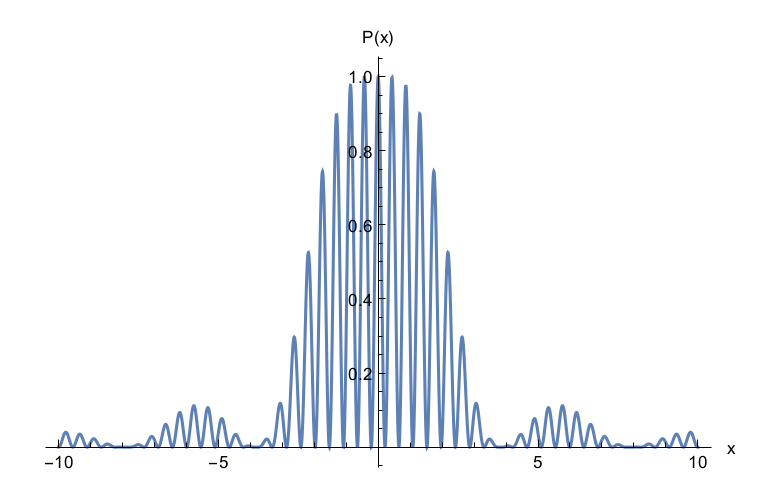
\includegraphics[width=.8\textwidth]{p.png}
  \caption{ The graph above shows the transition probability of spin
    down using Ramsey technique of separated oscillating fields. In
    this graph $T=8\tau$ and $ b \tau = \frac{\pi}{4}$. }
  \label{fig:transprob}
\end{figure}

An important special case of this relation is that corresponding to a
nuclear magnetic moment of spin-$\frac{1}{2}$ with gyromagnetic ratio
$\gamma$, in a fixed field of strength $B_0$, with a weak field of
strength $B_1$ perpendicular to $B_0$ and rotating about $B_0$. In
this case, the above equation applies with
\begin{align}
\omega_0 &= \gamma B_0 \, , \lambda=\omega_0 - \omega \\
2b &= \gamma B_1 =\frac{\omega_0 B_1}{B_0}
\end{align}
